\documentclass[11pt,twoside]{article}

\usepackage{amsmath}
\usepackage{amssymb}
\usepackage{amstext}

\usepackage[export]{adjustbox}

\usepackage{hyperref}
\usepackage{xcolor}
\hypersetup{
    colorlinks,
    linkcolor={red!50!black},
    citecolor={blue!50!black},
    urlcolor={blue!80!black}
}

\usepackage[english]{babel}

\usepackage{array}
\usepackage{tabularx,colortbl}
\usepackage{float}
\usepackage{listings}
\usepackage{color}

\usepackage[framemethod=tikz]{mdframed}
\usepackage{amsthm}

\definecolor{codegreen}{rgb}{0,0.6,0}
\definecolor{codegray}{rgb}{0.5,0.5,0.5}
\definecolor{codepurple}{rgb}{0.58,0,0.82}
\definecolor{backcolour}{rgb}{0.95,0.95,0.92}
 
\lstdefinestyle{mystyle}{
    backgroundcolor=\color{backcolour},   
    commentstyle=\color{codegreen},
    keywordstyle=\color{blue},
    numberstyle=\tiny\color{codegray},
    stringstyle=\color{red},
    identifierstyle=\color{black},
    basicstyle=\footnotesize,
    %breakatwhitespace=false,         
    breaklines=true,                 
    %captionpos=b,                    
    %keepspaces=true,                 
    numbers=left,                    
    numbersep=5pt,                  
    showspaces=false,                
    %showstringspaces=false,
    %showtabs=false,                  
    tabsize=4
}

\lstset{style=mystyle}



\newtheoremstyle{defi}
  {\topsep}%
  {\topsep}%
  {\normalfont}%
  {}%
  {\bfseries}% 
  {:}%
  {.5em}%
  {\thmname{#1}\thmnote{~(#3)}}%
\theoremstyle{defi}
\newmdtheoremenv{definitioni}{Definition}
\newmdtheoremenv[
hidealllines=true,
leftline=true,
innertopmargin=0pt,
innerbottommargin=0pt,
linewidth=4pt,
linecolor=gray!40,
innerrightmargin=0pt,
]{definitionii}{Definition}
\newmdtheoremenv[
roundcorner=5pt,
innertopmargin=0pt,
innerbottommargin=5pt,
linewidth=4pt,
linecolor=gray!40,
]{definitioniii}{Definition}


\usepackage[utf8]{inputenc}
\usepackage[a4paper, margin=2.5cm, top=3.5cm, bottom=1in]{geometry}

\renewcommand{\figurename}{Fig.}
\renewcommand{\tablename}{Tabla}

\definecolor{lightblue}{RGB}{135,206,250}


\title{
	  Algorithmics and Programming
}
\author{
Aleix Boné
}
\date{\today}

\setcounter{page}{-1}

\begin{document}
\topskip3cm
\clearpage\maketitle
\thispagestyle{empty}
\vspace{2cm}
\begin{center}
\begin{figure}[hb]
\centerline{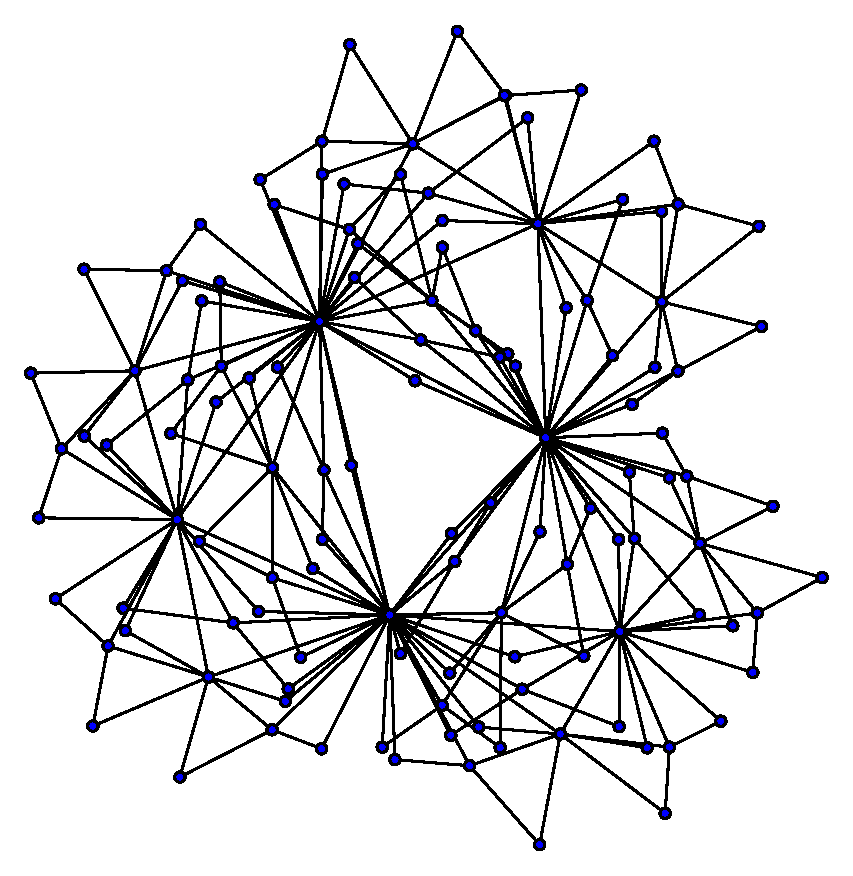
\includegraphics[width=0.7\textwidth]{src/DGMG.pdf}}
\end{figure}
\end{center}

\newpage
\mbox{}
\thispagestyle{empty}
\clearpage

\newpage
\topskip0pt
\tableofcontents
\newpage

\section{Base Conversion}

To convert a number $n$ from a base 10 to base $b$, we use chained divisions. The algorithm is as follows:
\begin{enumerate}
\item We take the number and divide it by $b$ and store the remainder $r_i$
	\item While the result of the division is different from 0, we apply the previous procedure.
	\item once we reach a quotient of 0, we take the remainders $r_i$ and the result will be those remainders in the form: $r_ir_{i-1}...r_1r_0$
\end{enumerate}

Following is a code in python to convert a number $n$ from base 10 to base $b$ (disregarding cases where $b>26$):

\begin{lstlisting}[language=Python]
def to_base_b(n,b):
	digits = "0123456789abcdefghijklmnopqrstuvwxyz"
	r = ""
	while (n!=0):
		r = digits[n% b] + r
		n//=b
	return r
\end{lstlisting}

To convert from a number $n$ to a base $b$, we first convert it to base 10 and then apply the method above. To convert it to base 10, we use the following formulae:
\begin{align}
(n)_b &= a_0a_1a_2...a_{s-1}a_s \notag \\
(n)_{10} &= \sum_{i=0}^sa_i*b^i
\end{align}

Following is a code in python that demonstrates the concept:

\begin{lstlisting}[language=Python]
def to_base_10(n,b):
	r = 0
	n = str(n)[::-1]
	for i in range(0,len(n)):
		d = n[i]
		if (d.isdigit()): d = int(d)
		else: d = ord(d)-ord('a')+10
		r+=b**i*d
	return r
\end{lstlisting}

\newpage

\section{Modular Arithmetic}

\begin{definitionii}
If a number $n\ \exists\ \mathbb{Z}$ gives a remainder $r$ when divided by a number $d\ \exists\ \mathbb{Z}$ then, we can express $n$ as : 
\begin{equation}
n = d*k +r
\end{equation}
For some number $k\ \exists\ \mathbb{Z}$.
We say that $n$ is congruent to $r$ in modulo $d$ if and only if $d|(n-r)$ (d divides $n-r$):
\begin{equation}
n \equiv r\ \ (mod\ d)
\end{equation}
\end{definitionii}

\subsection{Properties}
\begin{itemize}
\item If $a\ \equiv\ b\ \ (mod\ m)$, then both $a \& b$ have the same remainder when divided by $m$.
\subsubsection{Proof}
\begin{align*}
a &= k_1*m + r_1,\ b = k_2*m+r_2 \\
a-b&=(k_1-k_2)*m+r_1-r_2 \\
& \downarrow \\
& m | r_1-r_2 & 0 \leq r_1-r_2 < m \\
&\Downarrow\\
r_1-r_2&=0 \rightarrow r_1 = r_2
&&\boxtimes
\end{align*}

\item If $a\ \equiv\ b\ \ (mod\ m)$ \& $c\ \equiv\ d\ \ (mod\ m)$, then : $a\pm c\ \equiv\ b \pm d\ \ (mod\ m)$.
\subsubsection{Proof}
\begin{align*}
a &= k_1*m + b,\ c = k_2*m+d \\
a \pm c &= (k_1 \pm k_2)*m+b \pm d \\
& \Downarrow \\
a\pm c\ &\equiv\ b \pm d\ \ (mod\ m)
&&\boxtimes
\end{align*}

\item If $a\ \equiv\ b\ \ (mod\ m)$, then : $a*k\ \equiv\ b*k\ \ (mod\ m)\ \ \forall k\ \exists\ \mathbb{Z}$ .
\subsubsection{Proof}
\begin{align*}
a &= k_1*m + b\\
a * k &= k_1*k*m + b*k\\ 
& \Downarrow \\
a*k &\equiv\ b*k\ \ (mod\ m)
&&\boxtimes
\end{align*}

\item If $a\ \equiv\ b\ \ (mod\ m)$ \& $c\ \equiv\ d\ \ (mod\ m)$, then : $a*c\ \equiv\ b*d\ \ (mod\ m)$.
\subsubsection{Proof}
\begin{align*}
a &= k_1*m + b,\ c = k_2*m+d \\
a * c &= (k_1*m + b)*(k_2*m +d) &= k_1k_2m^2+ck_1m+bk_2m+bd \\ 
	  &= m*(mk_1k_2 + ck_1 + bk_2) + bd\\
& \Downarrow \\
a*c\ &\equiv\ b*d\ \ (mod\ m)
&&\boxtimes
\end{align*}

\item If $a\ \equiv\ b\ \ (mod\ m)$, then : $a^n\ \equiv\ b^n\ \ (mod\ m)\ \ \forall n\ \exists\ \mathbb{N}$ .
\subsubsection{Proof}
\begin{align*}
a &= k*m + b\\
a^n &= (km + b)^n &= \sum_{i=0}^n \binom{n}{i}*k^im^i*b^{n-i} \\
&= b^n+\sum_{i=1}^n \binom{n}{i}*k^im^i*b^{n-i} & m|\sum_{i=1}^n \binom{n}{i}*k^im^i*b^{n-i}\\
& \Downarrow \\
a^n\ &\equiv\ b^n\ \ (mod\ m)
&&\boxtimes
\end{align*}

\end{itemize}

\subsection{Inverse}\label{Inverse}

The inverse of $a$ must be a number $a^{-1}$ such that $a*a^{-1} \equiv 1\ \ (mod\ m)$. To find it, we can either try with all possible numbers from 0 to $m-1$ or we can express our congruence as a diophantine equation and find its solution. To solve the general inverse $a*a^{-1} = 1\ \ (mod\ m)$ we should solve the diophantine equation $a*a^{-1} + m*x =  1$

\subsection{Division rules}

\begin{itemize}
\item $1^{st}$ division rule:

If $a\ \equiv\ b\ \ (mod\ m)$, $d|a\ \&\ b$ and $gcd(d,m)=1$, then: $\frac{a}{d}\ \equiv\ \frac{b}{d}\ \ (mod\ m)$
\subsubsection{Proof}
\begin{align*}
a &= k*m + b\\
\frac{a}{d} &= m*\frac{k}{d} + \frac{b}{d} \\
& \Downarrow \\
\frac{a}{d}\ &\equiv\ \frac{b}{d}\ \ (mod\ m)
&&\boxtimes
\end{align*}

\item $2^{nd}$ division rule:

If $a\ \equiv\ b\ \ (mod\ m)$, $d|a\ \&\ b\ \& \ m$, then: $\frac{a}{d}\ \equiv \ \frac{b}{d}\ \ (mod\ \frac{m}{d})$
\subsubsection{Proof}
\begin{align*}
a &= k*m + b\\
\frac{a}{d} &= k*\frac{m}{d} + \frac{b}{d} \\
& \Downarrow \\
\frac{a}{d}\ &\equiv\ \frac{b}{d}\ \ \bigg( mod\ \frac{m}{d} \bigg)
&&\boxtimes
\end{align*}

\item $3^{rd}$ division rule:

If $a\ \equiv\ b\ \ (mod\ m)$, $d|a\ \&\ b$, then: $\frac{a}{d}\ \equiv \ \frac{b}{d}\ \ \big( mod\ \frac{m}{gcd(m,d)}\big)$
\subsubsection{Proof}
\begin{align*}
a &= k*m + b\\
\frac{a}{d} &= \frac{k*m}{d} + \frac{b}{d} = \frac{k*m}{\frac{gcd(d,m)}{gcd(d,m)}*d} + \frac{b}{d} = \frac{k*gcd(d,m)}{d}*\frac{m}{gcd(d,m)} + \frac{b}{d}\\
& \Downarrow \\
\frac{a}{d}\ &\equiv \ \frac{b}{d}\ \ \Bigg( mod\ \frac{m}{gcd(m,d)}\Bigg)
&&\boxtimes
\end{align*}

\end{itemize}

\subsection{Fermat's little theorem}
If $p$ is prime, and $a\ \exists\ \mathbb{Z}$, then, we get that:
\begin{align}
a^p &\equiv\ a\ \ (mod\ p)\\
a^{p-1} &\equiv\ 1\ \ (mod\ p)
\end{align}

\section{Linear congruences}
\begin{definitionii}
A linear congruence is a congruence in the form of an equation of degree 1. It can be expressed as:
$$ ax \equiv b\ \ (mod\ m)$$
Were $a,b,m\ \exists\ \mathbb{Z}$ and $x$ is a variable. Linear congruences can be solved using division rules and properties of congruences, but also, as seen in the special case of finding the inverse modulo $m$ (\ref{Inverse}) which is a linear congruence where $b=1$, a linear congruence can be solved using linear diophantine equations of the form:
$$ax + my = b$$
\end{definitionii}
Systems of simultaneous linear congruences can be solved using linear diophantine equations as many times as needed.
\subsection{Chinese remainder theorem}
If $m_1,m_2$ are co-prime ($gcd(m_1,m_2)=1$, then the simultaneous linear congruences:
$$x \equiv a_1\ (mod\ m_1),\ x \equiv a_2\ (mod\ m_2)\ \ldots\ x \equiv a_{m_1}\ (mod\ m_{n-1}),\ x \equiv a_n\ (mod\ m_n)$$
Have a \emph{unique} solution modulo ($\prod_{i=1}^nm_i$).

\section{Linear Diophantine equations}
\begin{definitionii}
A linear diophantine equation, is an equation of the form:
$$ ax+ by = c$$ 
Where $a,b,c\ \exists\ \mathbb{Z}$ and whose solution is of the form:
$$ x \equiv n_1\ \ (mod\ m_1),\ y \equiv\ n_2\ \ (mod\ m_2)$$ 
\end{definitionii}
To solve it, we use the result of the euclidean algorithm.
\subsection{Euclidean Algorithm}
\begin{definitionii}
The euclidean algorithm finds the gcd of two numbers $a,b$. To do so, we apply the following method:
\end{definitionii}
\begin{itemize}
\item if $b \neq 0$, then, $a=b,\ b=a (mod b)$
\item if $b = 0$, then the gcd of $a,b$ is $a$
\end{itemize}
Following is the one-line function that applies this method in c++:
\begin{lstlisting}[language=C++]
int gcd (int a, int b) { return (b)? gcd(b,a%b) : a; }
\end{lstlisting}
Similar function in python:
\begin{lstlisting}[language=python]
def gcd (a,b) : return gcd(b,a%b) if b else a
\end{lstlisting}

Using the results from the euclidean algorithm, we can say that:
$$ gcd = a_1-b_1*q_1 $$
and we can extend this until we get an expression as:
$$ gcd = k_1 * a + k_2 * b$$
And now we've got the solution for the linear diophantine equation.

\newpage
\section{Graph Theory}
\begin{definitionii}
A graph is formed by a set of vertices $\{V\}$ and a set of edges connecting those vertices $\{E\}$. Therefore:
$$G = \{V,E\}$$
\end{definitionii}
\begin{description}
\item[Vertex] a point of a graph which can be connected with edges
\item[Edge] line in a graph that connects 2 edges and can have a direction
\item[Adjacent] two vertices are adjacent if they are connected by an edge
\item[Faces] area delimited by at least 3 edges.
\item[Simple Graph] an undirected graph with no loops and no double edges.
\item[Directed Graph] a graph i which edges have a direction
\item[Loop] a edge connecting two the same vertex
\item[Multigraph] a graph with multiple edges between the same vertices
\item[Degree] the degree of a vertex is the number of edges that are connected to it. For a simple graph, the following condition is satisfied:
$$0\leq deg(V_i) \leq n-1$$
\item[Degree sequence] a sequence of all the degrees of a graph
\item[Connected Graph] A graph such that given any two vertices, there is a path that connects them. And therefore, it cannot be divided into two separate graphs without removing an edge.
\item[Complete graph] A simple graph where all vertices are joined by an edge, they are commonly referred by the letter $K$ and they have $\frac{1}{2}v(v-1)$ edges.
\item[Complementary graph] The graph $G'$ complementary to another graph $G$ is the same graph but with the edges swapped, meaning that if an edge existed in the complementary it doesn't and vice-versa. Thus, it will have $\frac{1}{2}v(v-1) - e$ edges.
\item[Bipartite graph] A graph that can be separated in two sets of vertices in which there are no connections between members of the same set.
\item[Tree] A simple connected acyclic graph
\item[Complete Bipartite graph] a bipartite graph with all the edges between the two sets of vertices, its usually refered as $K_{a,b}$ where $a,b$ are the number of vertices in each set.
\item[Planar Graph] a graph that can be represented in 2 dimensions without overlapping edges. It satisfies:
$$ e \leq 3v-6$$
\item[Sub-graph] A graph that is contained in another, meaning that if you remove some vertices from the original, you get the sub-graph.
\item[Minimum spanning tree] A subgraph that is a tree and connects all the vertices with the minimum weight possible
\end{description}

\begin{figure}
\caption{Complete graphs $K_n$ from $n = 3$ to $n = 12$}
    \centering
    \includegraphics[width=0.5\textwidth]{{"src/complete"}.pdf}
\end{figure}

\begin{figure}
\caption{Trees of 8 vertices}
    \centering
    \includegraphics[width=0.5\textwidth]{{"src/trees"}.pdf}
\end{figure}

\begin{figure}
\caption{Complete bipartite graph $K_{3,4}$}
    \centering
    \includegraphics[width=0.5\textwidth]{{"src/bipar"}.pdf}
\end{figure}

\newpage

\begin{description}
\item[Walk] Sequence of adjacent edges.
\item[Path] A walk with no repeated \emph{vertices}.
\item[Trail] A walk with no repeated \emph{edges}.
\item[Cycle] A closed path. (No repeated \emph{vertices})
\item[Circuit] A closed path. (No repeated \emph{edges})
\item[Hamiltonian cycle] A closed walk that uses each \emph{vertex} exactly once.
\item[Isomorphic graph] A graph that is equivalent to another graph even if its representation is similar, an isomorphic graph has same degrees and connections.
\item[Eulerian circuit] A closed walk that uses each \emph{edge} exactly once. So as to accomplish that, each vertex has to have even degree.
\item[Semi eulerian graph] A non-closed walk that uses each \emph{edge} exactly once. All vertices have to have even degree except 2 (the starting and ending vertices).
\end{description}

\subsection{Properties}
\subsubsection{Planar Graph}
\begin{align}
e &\leq 3v - 6 \\
f + v - e &= 2 
\end{align}
\subsubsection{Simple Graph}
\begin{equation}
e \leq \frac{3f}{2}
\end{equation}
\subsubsection{Tree}
\begin{equation}
e = v-1
\end{equation}

\subsection{Didac's theorem}
If a simple connected graph $G$ has $v$ vertices and all vertices have degree $\frac{v}{2}$, then $G$ is Hamiltonian.

\newpage

\subsection{Graph Algorithms}
\subsubsection{Kruskal algorithm}
\begin{definitionii}
Kruskal's algorithm is a greedy algorithm that finds the minimum spanning tree of a simple graph $G$
\end{definitionii}
The algorithm is as follows:
\begin{itemize}
\item Take the edge with minimum weight from the graph $G$ that is not already on our graph $T$.
\item If the edge doesn't form a cycle when connected, add it to $T$ otherwise discard it.
\item Repeat the previous steps until the graph $T$ contains $v-1$ edges.
\end{itemize}
Following is a simple implementation of the above algorithm extracted from a complete code that can be found in the annex (\ref{graphs.h}):
\lstinputlisting[language=C++, firstline=84, lastline=100, firstnumber=84]{src/graphs.h}
\begin{quote}
(To check is the new vertex forms a cycle, the best way is to use union sets although the above code uses a DFS for simplicity)
\end{quote}

\subsubsection{Check if bipartite}
To check if a graph is bipartite, we start at an arbitrary point and color it with the first colour $a$, we then colour all its adjacent vertices in the second colour $b$ and apply the same procedure on them, if we find one vertex that has two colour, the graph is \emph{not} bipartite otherwise it is bipartite.

\newpage

\subsubsection{Prim algorithm}
\begin{definitionii}
Prim's algorithm is a greedy algorithm that finds the minimum spanning tree of a simple graph $G$
\end{definitionii}
The algorithm is as follows:
\begin{itemize}
\item Take any arbitrary vertex of the graph
\item From all the vertices that we have visited, had to $T$ the edge with the minimum weight that connects to an unvisited vertex.
\item Repeat the previous step until the graph $T$ contains $v-1$ edges.
\end{itemize}
Following is a simple implementation of the above algorithm extracted from a complete code that can be found in the annex (\ref{graphs.h}):
\lstinputlisting[language=C++, firstline=102, lastline=121, firstnumber=102]{src/graphs.h}

\newpage

\subsubsection{Dijkstra}
\begin{definitionii}
Dijkstra’s algorithm is a greedy algorithm that finds the shortest path between any two vertices of a graph $G$ with no negative edges.
\end{definitionii}
The algorithm is as follows:
\begin{itemize}
\item Start at vertex $o$, label it with distance 0 and previous vertex $NULL$.
\item Add all the edges with the current distance plus the edges weight.
\item take the edge with the shortest distance that we have procesed and apply the above steps if the vertex we have reached has not yet been visited.
\item Repeat the previous steps until we reach vertex $b$ or we have checked all the vertices and found no path, so the graph is not connected and there is no possible path between the vertices.
\end{itemize}
Following is a simple implementation of the above algorithm extracted from a complete code that can be found in the annex (section \ref{graphs.h}) (an implementation of dijkstra with pointers can be found on annex section \ref{dijkstra_pointers}):
\lstinputlisting[language=C++, firstline=123, lastline=143, firstnumber=123]{src/graphs.h}

\newpage

\subsubsection{Chinese Postman problem}
\begin{definitionii}
Find the shortest circuit that goes through all edges (unlike an eulerian circuit, edges can be repeated).\end{definitionii}
We can do it easily if all the degrees are even (it has an eulerian circuit). If it has 2 vertices with odd degree, we must find the shortest path between those 2 (using Dijkstra or similar) and repeat the Dijkstra path. Similar approach can be applied if there are 4 vertices with odd degree (brute forcing which pairs to connect).

\subsubsection{Travelling salesman problem}
\begin{definitionii}
Find the shortest cycle that goes through all vertices (unlike a Hamiltonian circuit, vertices can be repeated).
\end{definitionii}
Only method is buy brute force (costs $1/2*(v-1)!$). Since the cost of the brute force is enormous, the best approach is to determine some lower and upper bounds ant take the best cycle found in some trials.

The simplest approach to find the upper and lower bounds consist of taking the $v$ smaller and bigger edges.

A better method to find the upper bound is to use the nearest neighbourhood algorithm (taking the nearest vertex that doesn't form a cycle until we have $v-1$ edges and the form the cycle).

A better method to find a lower bound is to remove a vertex and compute the minimum spanning tree of the resulting graph and finally add the two smaller edges of the removed vertex.

\newpage

\section{Recurrences}

\begin{definitionii}
A recurrence is a set of numbers $a_n$ defined in terms of other numbers of the recurrence or in terms of $n$
\end{definitionii}

A well known recurrence is the famous Fibonacci sequence defined as follows:
$$a_n = a_{n-1} + a_{n-2},\ a_0 = 1,\ a_1 = 1$$

\subsection{Homogeneous recurrences}
\begin{definitionii}
Linear Homogeneous recurrences with constant coefficients are recurrences which are defined only in terms of its previous elements (not in terms of n or with a constant). They have the form:

$$ a_n = c_1*a_{n-1} + c_2*a_{n-2} \ldots c_i*a_{n-i}$$

\end{definitionii}

To find the general solution of an homogeneous linear recurrence, we use the characteristic polynomial of the recurrence. To do so, we express the recurrence in terms of $a_n*t^n$ and factor out $t^{n-m}$. 

For an homogeneous recurrence:
$$a_n=\sum_{i=0}^m a_{n-i}*c_i$$
We define its characteristic polynomial as:
$$t^n = \sum_{i=0}^m t^{n-i}*c_i$$
And if we factor $t^{n-m}$, we get:
$$t^m = \sum_{i=0}^m t^{i}*c_i$$
Which is a polynomial which solutions $r_0,r_1 \ldots r_{m-1}, r_m $ can be used to determine $ a_n $ in the form:
$$a_n = \sum_{i=0}^m k_i*r_i^n$$
The factors $k_i$ can be determined using the base terms of the recurrence.

If some of the roots ($r_i$) have multiplicity bigger than one, then we have to multiply the root by the sum of$n^{\alpha_i-1-j}$ where $\alpha$ is the multiplicity of $r_i$ and $j$ ranges from 0 to $\alpha-1$. The solution then is as follows:
$$a_n = \sum_{i=0}^m \Bigg ( r_i^n* \sum_{j=0}^{\alpha_i-1}k_{i,j}*n^j \Bigg )$$

\newpage

\subsection{Non homogeneous recurrences}
\begin{definitionii}
Non homogeneous linear recurrences with constant coefficients are recurrences of the form:
$$ a_n = c_1*a_{n-1} + c_2*a_{n-2} \ldots c_i*a_{n-i} + f(n)$$
\end{definitionii}

We have two different methods to find the general solution of a non homogeneous recurrence, the first consists on subtracting recurrences to eliminate the non homogeneous part at the cost of increasing the degree of the characteristic polynomial resulting.

The second method consists on solving the recurrence only for the homogeneous part and then solving it for the non-homogeneous part knowing its form. The general solution will be the sum of the non-homogeneous and the homogeneous parts.

\newpage
\section{Annex}
\subsection{graphs.h}\label{graphs.h}
\lstinputlisting[language=C++]{src/graphs.h}
\subsection{Dijkstra with pointers}\label{dijkstra_pointers}
\lstinputlisting[language=C++]{src/Dijk.cpp}

\vspace{3cm}

\subsection{More Algorithms}
\begin{figure}[h]
    \caption{More Algorithms implemented in C++ can be found at: \url{https://github.com/Leixb/Cpp_algorithms}}
    \includegraphics[scale=0.5,center]{{"src/github"}.png}
\end{figure}

\end{document}